\documentclass[12pt]{standalone}
\usepackage[margin=1in]{geometry}
\usepackage{tikz}
\usetikzlibrary{shapes.geometric, arrows.meta, positioning}

% Define map styles
\tikzstyle{room} = [rectangle, draw=black, minimum height=2em, minimum width=6em, text centered, font=\footnotesize, align=center, inner sep=5pt]
\tikzstyle{arrow} = [thick,->,>=stealth]

\begin{document}

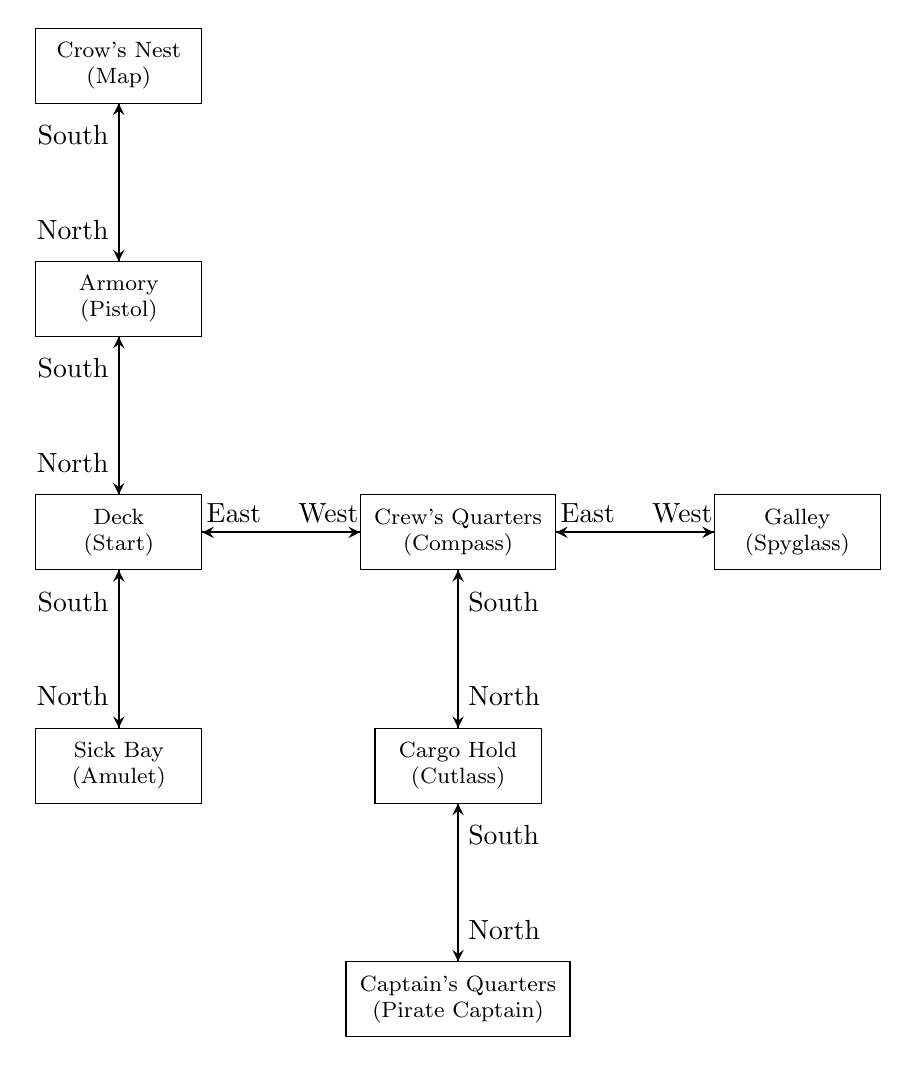
\begin{tikzpicture}[node distance=2cm and 2cm, auto]

% Nodes (Rooms)
\node[room] (deck) {Deck\\(Start)};
\node[room, right=of deck] (crew) {Crew’s Quarters\\(Compass)};
\node[room, right=of crew] (galley) {Galley\\(Spyglass)};
\node[room, below=of crew] (cargo) {Cargo Hold\\(Cutlass)};
\node[room, below=of cargo] (captain) {Captain’s Quarters\\(Pirate Captain)};
\node[room, below=of deck] (sickbay) {Sick Bay\\(Amulet)};
\node[room, above=of deck] (armory) {Armory\\(Pistol)};
\node[room, above=of armory] (crowsnest) {Crow’s Nest\\(Map)};

% Arrows (Connections)
\draw[arrow] (deck) -- node[pos=0.2, above] {East} (crew);
\draw[arrow] (crew) -- node[pos=0.2, above] {West} (deck);
\draw[arrow] (crew) -- node[pos=0.2, above] {East} (galley);
\draw[arrow] (galley) -- node[pos=0.2, above] {West} (crew);
\draw[arrow] (crew) -- node[pos=0.2, right] {South} (cargo);
\draw[arrow] (cargo) -- node[pos=0.2, right] {North} (crew);
\draw[arrow] (cargo) -- node[pos=0.2, right] {South} (captain);
\draw[arrow] (captain) -- node[pos=0.2, right] {North} (cargo);
\draw[arrow] (deck) -- node[pos=0.2, left] {South} (sickbay);
\draw[arrow] (sickbay) -- node[pos=0.2, left] {North} (deck);
\draw[arrow] (deck) -- node[pos=0.2, left] {North} (armory);
\draw[arrow] (armory) -- node[pos=0.2, left] {South} (deck);
\draw[arrow] (armory) -- node[pos=0.2, left] {North} (crowsnest);
\draw[arrow] (crowsnest) -- node[pos=0.2, left] {South} (armory);

\end{tikzpicture}

\end{document}